\documentclass[aspectratio=169]{beamer}
\usepackage{caption}        % caption in two lines
\usepackage{subcaption}
\usepackage[utf8]{inputenc} % codificacao de caracteres
\usepackage[T1]{fontenc}    % codificacao de fontes
\usepackage[brazil]{babel}  % idioma
\usepackage{graphicx}       %fundo
\usetheme{default}          % tema
\usecolortheme{orchid}     % cores
\usefonttheme[onlymath]{serif} % fonte modo matematico

\usepackage{subcaption}

\usepackage{listings}
\lstset{%frame=tb,
  language=C,
  aboveskip=3mm,
  belowskip=3mm,
  showstringspaces=false,
  columns=flexible,
  %basicstyle={\small\ttfamily},
  numbers=none,
  %numberstyle=\tiny\color{gray},
  %keywordstyle=\color{blue},
  %commentstyle=\color{dkgreen},
  %stringstyle=\color{mauve},
  breaklines=true,
  breakatwhitespace=true,
  tabsize=3
}

\beamertemplatenavigationsymbolsempty % Desativando os botoes de navegacao

% Tela cheia
\hypersetup{pdfpagemode=FullScreen}

% Titulo
\makeatletter
\newcommand\titlegraphicii[1]{\def\inserttitlegraphicii{#1}}
\titlegraphicii{}
\setbeamertemplate{title page}
{
  \vbox{}
   {\usebeamercolor[fg]{titlegraphic}\inserttitlegraphic\hfill\inserttitlegraphicii\par}
  \begin{centering}
    \begin{beamercolorbox}[sep=2pt,center]{institute}
      \usebeamerfont{institute}\insertinstitute
    \end{beamercolorbox}
    \begin{beamercolorbox}[sep=12pt,center]{title}
      \usebeamerfont{title}\inserttitle\par%
      \ifx\insertsubtitle\@empty%
      \else%
        \vskip0.2em%
        {\usebeamerfont{subtitle}\usebeamercolor[fg]{subtitle}\insertsubtitle\par}%
      \fi%     
    \end{beamercolorbox}%
    \vskip0.2em\par
    \begin{beamercolorbox}[sep=2pt,center]{author}
      \usebeamerfont{author}\insertauthor
    \end{beamercolorbox}
    %\begin{beamercolorbox}[sep=4pt,center]{date}
      %\usebeamerfont{date}\insertdate
    %\end{beamercolorbox}%\vskip0.5em
  \end{centering}
  %\vfill
}
\makeatother
\title{INTERPRETAÇÃO DOS DIALETOS RS274-D E EXTRAÇÃO DOS DADOS
TEMPORAIS DA USINAGEM EM MÁQUINAS CNC}
%\subtitle{Subtítulo}
\author{\textbf{Francisco Ricardo Taborda Aguiar}}
\institute{UNIVERSIDADE FEDERAL DO PARANÁ \\ 
PROGRAMA DE PÓS GRADUAÇÃOEM ENGENHARIA DE MANUFATURA \\
MESTRADO PROFISSIONAL EM ENGENHARIA DE MANUFATURA} % opcional


\AtBeginSubsection[]
{
  \begin{frame}<beamer>{Assuntos}   
    \tableofcontents[currentsection,currentsubsection]
  \end{frame}
}

% Let's get started
\begin{document}
{%
 \usebackgroundtemplate{
  \centering
  
\includegraphics[width=\paperwidth]{CapaUFPR.png}
 }
\begin{frame}
  \titlepage
\end{frame}
}
{%
 \usebackgroundtemplate{
  \centering
  
\includegraphics[width=\paperwidth]{FundoUFPR2.png}
 }
\begin{frame}{Assuntos}
  \tableofcontents
  % You might wish to add the option [pausesections]
\end{frame}

% Section and subsections will appear in the presentation overview
% and table of contents.

\section{Introdução}

\begin{frame}
  \frametitle{Introdução}

  TODO

\end{frame}

\section{Formatos}


\subsection{Padrão RS274-D}

\begin{frame}{Origem}
  \begin{itemize}
  \item {
    Nos anos sessenta, a Electronic Industry Association (EIA) desenvolveu um 
    padrão conhecido como RS274-D para programar máquinas CNC.
  }
  \item {
    A mídia de armazenamento comum era baseada nos cartões perfurados.
  }
  \item {
    Hardware restrito.
  }
  \item {
    Caracteres representados no padrão ASCII (American Standard Code for Information Interchange).
  }
  \item {
    Em 1982 o padrão foi adotado pela ISO sendo chamado de ISO 6983.
  }
  \item {
    O arquivo descreve o percurso da ferramenta com relação aos eixos.
  }
  \end{itemize}
\end{frame}

%\subsection{Objetivos}

\begin{frame}{Objetivos}
  \begin{itemize}
  \item {
    Promover a uniformidade de técnicas de programação.
  }
  \item {
    Favorecer a intercambiabilidade de programas entre diferentes máquinas de controle numérico.
  }
  \item {
    Máquinas simples possam ser programadas com um formato simples de programa,
    o qual possa se extensível para máquinas mais complexas.
  }
  \end{itemize}
\end{frame}

%\subsection{Arquitetura}

\begin{frame}{Arquitetura}
  \begin{itemize}
  \item {
    Os programas são organizados em linhas de código, também chamados de blocos.
  }
  \item {
    Um bloco consiste de um número de linha opcional no início do bloco, seguido por um 
    ou mais comandos.
  }
  \item {
    Um comando (ou palavra) corresponde a uma letra sucedida por um sinal algébrico, se aplicável, 
    seguido por um número ou por uma expressão que pode ser avaliada para um número.
  }
  \end{itemize}
\end{frame}

\begin{frame}{Comandos}
  \begin{itemize}
  \item {
    Os comandos devem ser apresentados na seguinte sequência dentro do bloco.
    \begin{itemize}
      \item Os comandos de preparação G;
      \item Os comandos de dimensão, arranjadas na seguinte sequência: X,
      Y, Z, U, V, W P, Q, R, A, B, C.
      \item Os comandos de interpolação I, J e K, aplicáveis somente para determinados 
      grupos de eixos.
      \item O comando para a função de avanço F.
      \item O comando para a função de velocidade de corte S.
      \item O comando para a função de ferramenta T.
      \item O comando para a função de miscelânea.
    \end{itemize}
  }
  \end{itemize}
\end{frame}

\begin{frame}{Exemplos de alguns comandos RS274/NGC}

  \scriptsize{Fonte: KRAMER, T.; PROCTOR, F. 
    The NIST RS274/VGER Interpreter. US Department of
    Commerce, National Institute of Standards e Technology, set. 1998.}

  \begin{table}[H]
    \centering
    \begin{tabular}{p{7cm}|p{5cm}}
    
      \hline
      \bfseries{\scriptsize{Comandos}} & \bfseries{\scriptsize{Prop\'osito}} \\
  
      \hline
      \scriptsize{G0, G1, G2, G3, G38, G80, G81, G82, G83, G84, G85, G86, G87, G88, G89} 
      & \scriptsize{Movimento} \\
  
      \hline
      \scriptsize{G17, G18, G19} 
      & \scriptsize{Sele\c c\~ao do plano} \\
  
      \hline
      \scriptsize{G90, G91}
      & \scriptsize{Modo das dist\^ancias} \\
  
      \hline
      \scriptsize{G93, G94}
      & \scriptsize{Modo da velocidade de corte} \\
  
      \hline
      \scriptsize{G20, G21}
      & \scriptsize{Unidade} \\
  
      \hline
      \scriptsize{G40, G41, G42}
      & \scriptsize{Compensa\c c\~ao do di\^ametro de corte} \\
  
      \hline
      \scriptsize{G43, G49}
      & \scriptsize{Dist\^ancia da ferramenta} \\
  
      \hline
      \scriptsize{G98, G99}
      & \scriptsize{Modo de retorno em ciclos fixos} \\
  
      \hline
      \scriptsize{G54, G55, G56, G57, G58, G59, G59.1, G59.2, G59.3}
      & \scriptsize{Sele\c c\~ao do sistema de coordenadas} \\
  
      \hline
      \scriptsize{M0, M1, M2, M30, M60}
      & \scriptsize{Parada} \\
  
      \hline
      \scriptsize{M6}
      & \scriptsize{Troca de ferramenta} \\
  
      \hline
      \scriptsize{M3, M4, M5}
      & \scriptsize{Sentido do giro do eixo} \\
  
      \hline
      \scriptsize{M7, M8, M9}
      & \scriptsize{Refrigera\c c\~ao} \\
  
      \hline
      \scriptsize{M48, M49}
      & \scriptsize{Interruptor do avan\c co e do corte} \\

      \hline
  
    \end{tabular}
  \end{table}

\end{frame}

%\section{Dialetos RS274-D}

%\subsection{Problema}

\begin{frame}{Dialetos}
  \begin{itemize}
  \item {
    Os padrões são apenas nominais hoje em dia.     
  }
  \item {   
    A tecnologia dos sistemas CNC avançou muito desde que as normas foram publicadas.
  }
  \item {
    Os fabricantes de máquinas têm estendido o padrão (base comum). 
  }
  \end{itemize}
\end{frame}


%\subsection{Dialetos: Exemplos}

\begin{frame}{Exemplos}
  \begin{itemize}
    \item {
      Fonte: Adaptado de ZHANG, X.; NASSEHI, A.; NEWMAN, S. T. A meta-model of computer numerical
      controlled part programming languages. Proceedings of the Institution of
      Mechanical Engineers, Part B: Journal of Engineering Manufacture, Sage
      Publications Sage UK: London, England, v. 229, n. 7, p. 1243–1257, 2015.
      \begin{table}[H]
        \centering    
        {\begin{tabular}{p{4.3cm}|p{2.6cm}|p{2.4cm}}
          \hline
          \bfseries{\footnotesize{Comando}} & 
          \bfseries{\footnotesize{Fanuc}} & 
          \bfseries{\footnotesize{Siemens}} \\
      
          \hline
          \footnotesize{Interpolação Linear} & 
          \footnotesize{G01 X...Y...} & 
          \footnotesize{G1 X...Y...} \\
      
          \hline
          \footnotesize{Interpolação Circular (Horário)} & 
          \footnotesize{G02 X...Y...I...J...} & 
          \footnotesize{G2 X...Y...I...J...} \\
      
          \hline
          \footnotesize{Ciclo Fixo de Furação} & 
          \footnotesize{G83...} & 
          \footnotesize{CYCLE G83...} \\
      
          \hline
          \footnotesize{Definição da Unidade} & 
          \footnotesize{G20 ou G21 } & 
          \footnotesize{G70 ou G71} \\

          \hline

        \end{tabular}}
      \end{table}
    }    
  \end{itemize}
\end{frame}


\subsection{Padrão STEP-NC}

\begin{frame}{Origem}
  \begin{itemize}
  \item {
    Esforço realizado pelo Comitê Técnico da ISO 184 (Sistemas de Automação Industrial e
    Integração) para enfrentar o problema com interoperabilidade e integração.
  }
  \item {
    Formalizado na norma ISO 10303 (Padrão Internacional para a representação e troca de dados do produto).
  }  
  \item {
    O padrão ISO 14649 (STEP-NC) define um modelo para a transferência de dados entre sistemas CAD/CAM.
  }
  \item {
    Correspode a um modelo mais completo de informações para descrever processos de usinagem.
    \begin{itemize}
      \item A geometria da peça.
      \item Os features da usinagem.
      \item A sequência de operações.
      \item Os parâmetros de processo.
      \item As especificações de ferramentas.
    \end{itemize}
  }
  \end{itemize}
\end{frame}

%\subsection{Objetivos}

\begin{frame}{Objetivos}
  \begin{itemize}
    \item {
      Substituir o padrão RS274-D / ISO 6983.
    }
    \item{
      A criação de um padrão internacional que seja único capaz de cobrir todos os aspectos 
      da transferência de dados entre sistemas CAD/CAM.
    }
    \item {
      A padronização de um mecanismo para descrever os dados do produto, ao longo do ciclo de 
      vida do produto.
    }
    \item {
      Formato neutro para a troca de dados.
    }
    \item {
      Fazer a separação entre a descrição do produto e a sua implementação, 
      de forma independente de sistemas particulares.
    }
    \item {
      Capaz de fornecer as bases para o compartilhamento de bancos de dados de produtos.
    }
  \end{itemize}
\end{frame}


%\subsection{Exemplo}

\begin{frame}{Exemplo}

  Adaptado de POBOZNIAK, J.; SOBIESKI, S. Extension of STEP-NC data structure to represent
  manufacturing process structure in CAPP system. Procedia Manufacturing, Elsevier,
  v. 11, p. 1692-1699, 2017.

  \begin{figure}[H]
    \centering
    \begin{subfigure}[b]{0.46\textwidth}
        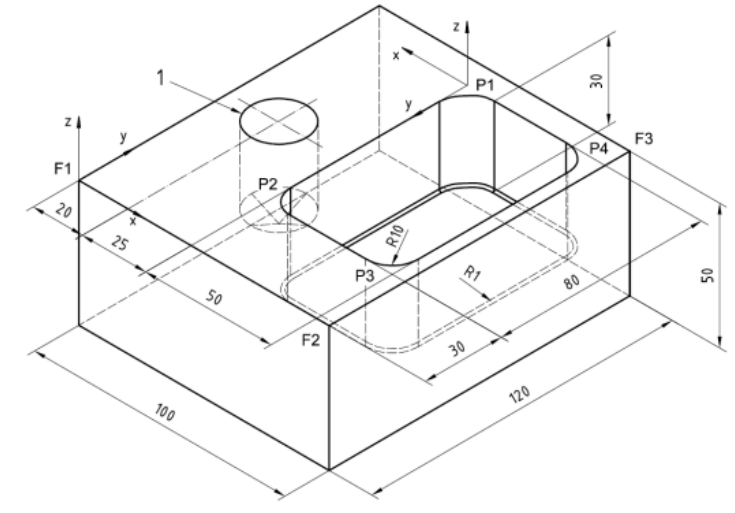
\includegraphics[width=\textwidth]{part1.png}
    \end{subfigure}
    \qquad
    \begin{subfigure}[b]{0.46\textwidth}
        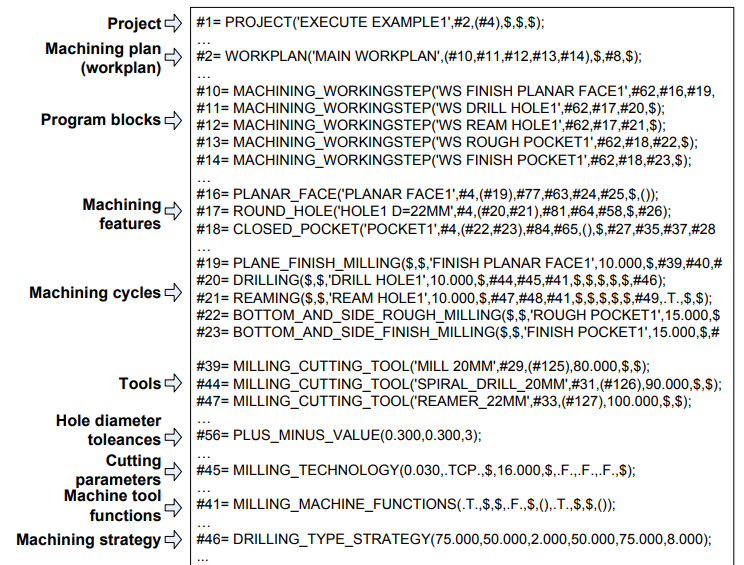
\includegraphics[width=\textwidth]{step-nc-sample-1.png}
    \end{subfigure}
\end{figure}

\end{frame}

%\subsection{Problema}

\begin{frame}{Considerações}

  \begin{itemize}
    \item {
      Apesar do interesse em torno do formato STEP-NC e da inovação tecnológica
      que vem acontecendo nos equipamentos de CNC, o formato RS274-D ainda é dominante.
    }
    \item {
      Os processos de usinagem ainda dependem de máquinas antigas controladas
      por sistemas NC proprietários que são dialetos das normas RS274-D ou ISO 6983.
    }
  \end{itemize}   

\end{frame}


\subsection{Funções Canônicas de Usinagem}

\begin{frame}{Funções Canônicas de Usinagem}
  \begin{itemize}
    \item{
      A Intelligente Systems Division (ISD) do National Institute of Standards and Technology (NIST) 
      trabalhou no projeto Enhanced Machine Controller (EMC), de forma colaborativa com outros parceiros.
    }
    \item {
      O objetivo do projeto foi construir um padrão de interface de programação de aplicações 
      (API) para controladores de máquinas com arquitetura aberta. 
      Além disto, demonstrar as implementações da arquitetura do Next Generation Controller (NGC).
    }
    \item {
      A arquitetura NGC utiliza a linguagem RS274/NGC, um dialeto do padrão RS274-D.
    }
    \item {
      O interpretador RS274/VGER foi desenvolvido pelo NIST para converter programas escritos no dialeto 
      RS274/NGC para Funções Canônicas de Usinagem.
    }
  \end{itemize}
\end{frame}


\begin{frame}{Funções Canônicas de Usinagem: Objetivos}
  \begin{itemize}    
    \item {
      As Funções Canônicas de Usinagem (do Inglês, CMF, Canonical Machining Functions)
      foram projetadas com três objetivos em mente.
      \begin{itemize}        
        \item {
          Todas as funcionalidades dos centros de usinagem de 3 a 6 eixos devem ser
          cobertas pelos comandos.
        }
        \item {
          Os comandos canônicos de movimento devem ser portáveis para serem 
          reconhecidos em placas de controle comerciais disponíveis no mercado.         
        }
        \item {
          Deve ser possível interpretar comandos RS274-D em chamadas de 
          Funções Canônicas de Usinagem.
        }
      \end{itemize}
    }
    \item {
      O projeto EMC e outros projetos abertos de pesquisa em máquinas CNC utilizam CMFs.
    }
    \item {
      As Funções Canônicas de Usinagem consistem em comandos atômicos.
      Os comandos RS274-D podem ser decompostos em várias chamadas de CMFs.
    }
  \end{itemize}
\end{frame}


\begin{frame}{Funções Canônicas de Usinagem: Exemplos de comandos}
  \begin{table}[H]
    \centering
    \begin{tabular}{p{7cm}|p{5cm}}

      \hline
      \bfseries{\scriptsize{Comandos}} & \bfseries{\scriptsize{Prop\'osito}} \\

      \hline  
      \scriptsize{SET\_TRAVERSE\_RATE (double \emph{rate})} 
      & \scriptsize{Define o valor superior da velocidade do movimento de aproxima\c c\~ao 
      que ser\'a utilizado durante os movimentos r\'apidos que ocorrem, normalmente, quando 
      o equipamento n\~ao est\'a fazendo opera\c c\~oes de corte.} \\

      \hline      
      \scriptsize{STRAIGHT\_TRAVERSE (double \emph{x}, double \emph{y}, double \emph{z}, 
      double \emph{a}, double \emph{b}, double \emph{c})} 
      & \scriptsize{Faz um movimento de posicionamento linear a partir da posi\c c\~ao 
      atual at\'e o ponto definido por \emph{x}, \emph{y}, \emph{z}, \emph{a}, \emph{b} e \emph{c}.
      \'E esperado que n\~ao ocorra opera\c c\~ao de corte durante o movimento de travessia.} \\

      \hline  
      \scriptsize{SET\_FEED\_RATE (double \emph{rate})}
      & \scriptsize{Define a velocidade de avan\c co.} \\

      \hline  
      \scriptsize{STRAIGHT\_FEED (double \emph{x}, double \emph{y}, double \emph{z}, 
      double \emph{a}, double \emph{b}, double \emph{c})} 
      & \scriptsize{Move em linha reta, na velocidade de avan\c co previamente definida, 
      a partir da posi\c c\~ao atual at\'e a 
      posi\c c\~ao dada por \emph{x}, \emph{y} e \emph{z}.} \\

      \hline  
      \scriptsize{SET\_SPINDLE\_SPEED (double \emph{speed})} 
      & \scriptsize{Define a velocidade de rotação} \\

      \hline

    \end{tabular}
  \end{table}
\end{frame}


\begin{frame}{Considerações}

  \begin{itemize}
    \item Assim como ocorre com o \emph{STEP-NC}, o formato baseado nas 
          Funções Canônicas de Usinagem não tem sido amplamente adotado 
          entre os controladores de CNC comerciais.
    \item A atomicidade das Funções Canônicas de Usinagem representa uma 
          característica interessante para o registro temporal de cada 
          evento que ocorre na máquina-ferramenta durante o processamento 
          do programa.
    \item A simplicidade da sintaxe e a padronização das chamadas de 
          funções são pontos positivos para a construção de uma camada 
          de abstração a partir das Funções Canônicas de Usinagem.
    \emph{CN}.

  \end{itemize}

\end{frame}


\section{Projeto proposto}

\subsection{Objetivo}

\begin{frame}{Objetivo Geral}
  \begin{itemize}
    \item { 
      Desenvolver uma metodologia para interpretar os diferentes dialetos 
      do formato \emph{RS274-D} e gerar um modelo granular de dados, no qual 
      cada movimento da m\'aquina \'e registrado com uma marcação de tempo.
    }
  \end{itemize}
\end{frame}

\begin{frame}{Objetivos Específicos}
  \begin{itemize}
    \item Projetar uma estrutura de dados que contemple dois objetivos:
    \begin{itemize}
        \item Possibilitar o registro temporal dos eventos decorrentes do 
              processamento do programa de controle numérico.
        \item Formar uma camada abstrata de dados que possa ser utilizada
              para tratar das questões da interoperabilidade entre os 
              dialetos.
    \end{itemize}
    \item Representar, por meio de diagramas abstratos, a metodologia proposta na dissertação.
    \item Implementar um estudo de caso a partir de um dialeto específico.
\end{itemize}
\end{frame}


\subsection{Metodologia}

\begin{frame}{Módulos}
  \begin{enumerate}
    \item {
      \emph{Transpiler}: 
      \begin{itemize}
        \item Interpretar o formato \emph{RS274-D};
        \item Adaptável aos diversos dialetos RS274-D;
        \item Elevar o nível de abstração dos dados para um formato 
              neutro (independente de tecnologias proprietárias).
        \item Processar o formato neutro e gerar as marcações de tempo.
      \end{itemize}
    }

    \item {
      \emph{Persistence}:
      \begin{itemize}
        \item Armazenar e restaurar os dados do tipo \emph{Payload}.
        \item Foi definida uma arquitetura orientada a documentos 
              (\emph{NoSQL}) para o banco de dados, pois o sistema 
              proposto não apresenta uma natureza relacional.
      \end{itemize}
    }

    \item {
      \emph{Output}
      \begin{itemize}
        \item Interpretar a lista de objetos \emph{Payload} 
              e gerar dois tipos de saída:
        \begin{itemize}
              \item Um arquivo com os dados temporais da usinagem. 
                    Em formato \emph{CSV}, para facilitar a importação 
                    do arquivo em softwares de análise de dados.
              \item Um arquivo em formato de Funções Canônicas de Usinagem.
        \end{itemize}
      \end{itemize}
    }

  \end{enumerate}
\end{frame}

TODO

\begin{frame}{Interpretação}
  \begin{itemize}
    \item Abordagem baseada em um fluxo de duas etapas:
    \begin{enumerate}
      \item Análise Léxica (ou \emph{Scanning}).
      \item Análise Sintática (ou \emph{Parsing}).
    \end{enumerate}
  \end{itemize}
\end{frame}


\begin{frame}{Interpretação: Etapa 1}
  \begin{itemize}
    \item A primeira etapa (\emph{Scanner}) l\^e a entrada e traduz as 
          cadeias de caracteres em símbolos (tokens). 
    \item Uma ferramenta chamada \emph{Flex} foi utilizada para esta 
          implementa\c c\~ao.
    \item Os tokens são identificados a partir de Expressões Regulares.
  \end{itemize}
\end{frame}


\begin{frame}[fragile]
  \frametitle{Interpretação: Exemplo de Expressões Regulares}
  \begin{example}
      "G1X10.Y3.5Z-1.F505"
      \begin{lstlisting}
        GCODE = 'G'        
        INT = '[0-9]+'
        X = '[Xx]'
        Y = '[Yy]'
        Z = '[Zz]'
        F = 'F'
        FLOAT = '[+-]?[0-9]+[.]?[0-9]*'
      \end{lstlisting}
    \end{example}
  \end{frame}


  \begin{frame}
    \frametitle{Detalhamento da Expressão Regular \emph{FLOAT}}
    \begin{itemize}
      \item \emph{FLOAT} = \emph{'[+-]?[0-9]+[.]?[0-9]*'}
        \begin{itemize}
          \item \emph{[-+]}: um caractere \emph{+} ou \emph{-}.
          \item \emph{?}: o caractere anterior (no caso, \emph{+} ou \emph{-}) deve aparecer 0 ou 1 vez.
          \item \emph{[0-9]}: um dígito (de 0 até 9).
          \item \emph{+}: o caractere anterior (no caso, um dígito) deve aparecer 1 ou mais vezes.
          \item \emph{[.]}: um ponto final (\emph{.}).
          \item \emph{?}: o caractere anterior (no caso, um ponto final) deve aparecer 0 ou 1 vez.
          \item \emph{[0-9]}: um dígito (de 0 até 9).
          \item \emph{*}: o caractere anterior (no caso, um dígito) deve aparecer 0 ou muitas vezes.
      \end{itemize}
    \end{itemize}
\end{frame}


\begin{frame}{Interpretação: Etapa 2}
  \begin{itemize}
    \item A segunda etapa (\emph{Parser}) agrupa os símbolos em unidades 
          sint\'aticas (no caso, blocos de comandos).
    \item Utiliza uma Gramática Livre de Contexto (Context-Free Grammar).
    \item Consiste em um conjunto de regras gramaticais que descrevem a 
          sintaxe de uma determinada linguagem (no caso, um dialeto RS274-D).
    \item Extensível para os diversos dialetos.
    \item A sintaxe do dialeto é descrita através da notação Backus-Naur 
          Form (BNF).
    \begin{itemize}
      \item Linguagens de programação, formatos de documentos e 
            protocolos de comunicação.
    \end{itemize}
    \item O processamento é feito por um algoritmo \emph{LR}, baseado no método 
          \emph{Shift-Reduce}, amplamente utilizado para o processamento 
          de linguagens de computação.
  \end{itemize}
\end{frame}


\begin{frame}[fragile]
  \frametitle{Interpretação: Exemplo de Especificação BNF}
  \begin{example}
   "G1X10.Y3.5Z-1.F505"
    \begin{lstlisting}
      machining : GCODE "1" position F INT

      position : X FLOAT
               | Y FLOAT
               | Z FLOAT
               | X FLOAT Y FLOAT
               | X FLOAT Z FLOAT
               | Y FLOAT Z FLOAT
               | X FLOAT Y FLOAT Z FLOAT
    \end{lstlisting}
  \end{example}  
\end{frame}


\begin{frame}{Abstração}
  \begin{itemize}
    \item Formato de dados escolhido: Funções Canônicas de Usinagem.
    \begin{itemize}
      \item Formato Padronizado.
      \item Capaz de descrever cada movimento feito durante a usinagem.
    \end{itemize}
    \item Modelagem Orientada a Objetos.
  \end{itemize}
\end{frame}


\begin{frame}{Abstração: Modelo Orientado a Objetos}
  Fonte: Autor.
  \begin{figure}[H]
    \centering
    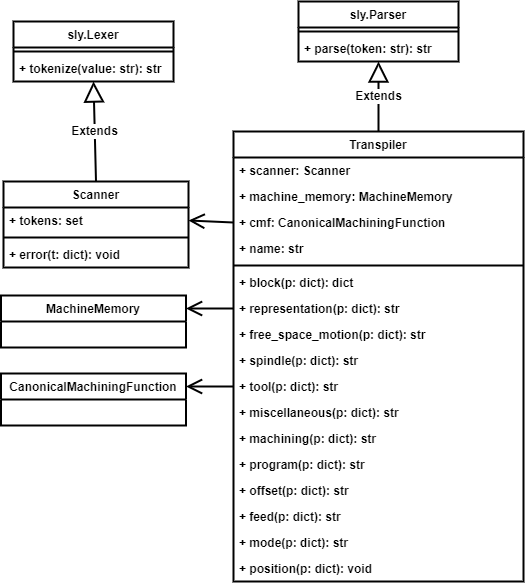
\includegraphics[width=6.2cm]{ncparser-class-transpiler.png}
  \end{figure}
\end{frame}


\begin{frame}{Abstração: Modelo Orientado a Objetos}
  Fonte: Autor.
  \begin{figure}[H]
    \centering
    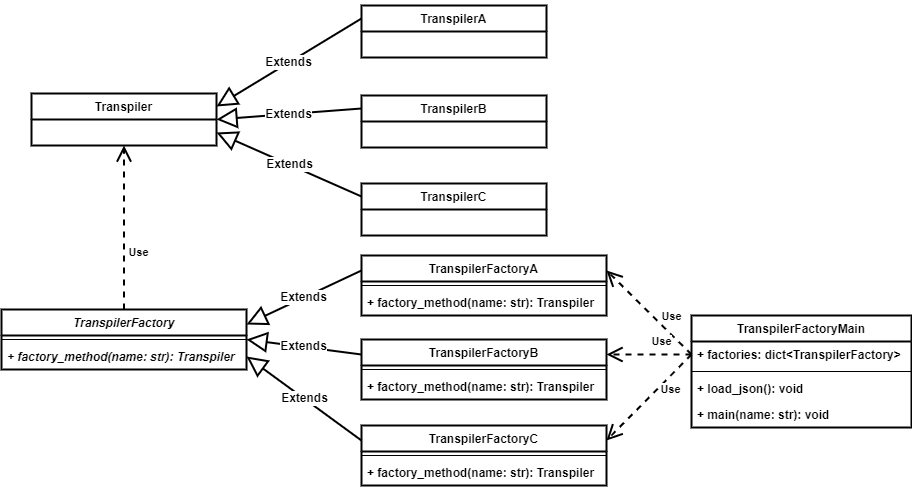
\includegraphics[width=10.5cm]{ncparser-class-transpiler-factory.png}
  \end{figure}
\end{frame}


\begin{frame}{Abstração: Exemplo de Transpilação para Funções Canônicas de Usinagem}
  \scriptsize{Fonte: Autor.}
  \begin{table}[H]
    \centering
    \begin{tabular}{ |l|l| } 
      \hline
      \tiny{\bfseries{Mach9}} & \tiny{\bfseries{Funções Canônicas de Usinagem}} \\
      \hline
      \tiny{O3S1857M3} & \tiny{SET\_SPINDLE\_SPEED(1857.0)} \\
      & \tiny{START\_SPINDLE\_CLOCKWISE()} \\
      \hline
      \tiny{G0X-15.Y-65.Z3.} & \tiny{STRAIGHT\_TRAVERSE(-15.0, -65.0, 3.0)} \\
      \hline
      \tiny{X-15.Y-65.Z5.} & \tiny{STRAIGHT\_TRAVERSE(-15.0, -65.0, 5.0)} \\
      \hline
      \tiny{G81Z-8.R3.F186} & \tiny{STRAIGHT\_TRAVERSE(-15.0, -65.0, 3.0)} \\
      \tiny{G25X30.Y130.I2J2} & \tiny{SET\_FEED\_RATE(186.0)} \\
      \tiny{G80} & \tiny{STRAIGHT\_FEED(-15.0, -65.0, -8.0)} \\
      & \tiny{STRAIGHT\_TRAVERSE(-15.0, -65.0, 3.0)} \\
      & \tiny{STRAIGHT\_TRAVERSE(15.0, -65.0, 3.0)} \\
      & \tiny{SET\_FEED\_RATE(186.0)} \\
      & \tiny{STRAIGHT\_FEED(15.0, -65.0, -8.0)} \\
      & \tiny{STRAIGHT\_TRAVERSE(15.0, -65.0, 3.0)} \\
      & \tiny{STRAIGHT\_TRAVERSE(15.0, 65.0, 3.0)} \\
      & \tiny{SET\_FEED\_RATE(186.0)} \\
      & \tiny{STRAIGHT\_FEED(15.0, 65.0, -8.0)} \\
      & \tiny{STRAIGHT\_TRAVERSE(15.0, 65.0, 3.0)} \\
      & \tiny{STRAIGHT\_TRAVERSE(-15.0, 65.0, 3.0)} \\
      & \tiny{SET\_FEED\_RATE(186.0)} \\
      & \tiny{STRAIGHT\_FEED(-15.0, 65.0, -8.0)} \\
      & \tiny{STRAIGHT\_TRAVERSE(-15.0, 65.0, 3.0)} \\
      \hline    
    \end{tabular}    
  \end{table}
\end{frame}


\begin{frame}{Processamento}
  \begin{itemize}
    \item Processar as Funções Canônicas.
    \begin{itemize}
      \item As Fun\c c\~oes Can\^onicas de Usinagem consiste em um formato padronizado (API).
      \item Comandos atômicos.
    \end{itemize}
    \item Gerar o arquivo com as marcações de tempo.
  \end{itemize}
\end{frame}

\begin{frame}{Processamento}
  \begin{itemize}
    \item Expressões Regulares para extrair os símbolos.
    \item Gramática Livre de Contexto + Algoritmo LR para processar.
    \item Abordagem Orientada a Objetos.
  \end{itemize}
\end{frame}


\begin{frame}[fragile]
  \frametitle{Processamento: Exemplo de Expressão Regular}
    \begin{example}
      STRAIGHT\_FEED(10.0, 3.5, -1.0)
        \begin{lstlisting}
          LPAR = '('
          RPAR = ')'    
          DOUBLE = '[+-]?[0-9]+[.]?[0-9]*'
          INT = '[0-9]+'
          COMMA = '[,]\s*'
        \end{lstlisting}
      \end{example}
\end{frame}


\begin{frame}[fragile]
  \frametitle{Processamento: Exemplo de Especificação BNF}
  \begin{example}
    STRAIGHT\_FEED(10.0, 3.5, -1.0)
    \begin{lstlisting}[basicstyle=\tiny]
      machining : "STRAIGHT_FEED" LPAR position RPAR

      position : DOUBLE COMMA DOUBLE COMMA DOUBLE
               | DOUBLE COMMA DOUBLE COMMA DOUBLE COMMA DOUBLE COMMA DOUBLE COMMA DOUBLE
    \end{lstlisting}
  \end{example}  
\end{frame}


\begin{frame}{Processamento: Modelo Orientado a Objetos}
  Fonte: Autor.
  \begin{figure}[H]
    \centering
    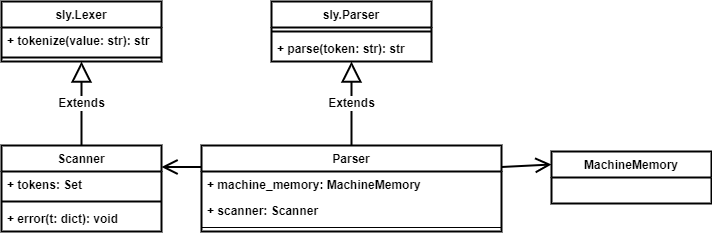
\includegraphics[width=11.0cm]{ncparser-class-canonical-parser.png}
  \end{figure}
\end{frame}


\subsection{Estudo de Caso}

\begin{frame}
  \frametitle{Estudo de Caso}

    TODO

\end{frame}


\subsection{Conclusão}

\begin{frame}
  \frametitle{Conclusão}

    TODO

\end{frame}


\end{document}


% Transpila\c c\~ao (ou transcompila\c c\~ao, ou compila\c c\~ao de fonte para fonte) refere-se ao processo de 
% tradu\c c\~ao de c\'odigo-fonte escrito em uma determinada linguagem para uma outra. Portanto, o transcompilador 
% \'e um tipo especial de compilador.


% Para o desenvolvimento do transpilador foi utilizada uma abordagem baseada em An\'alise Sint\'atica 
% (comumente encontrada em compiladores) e um modelo orientado a objetos.
% O algoritmo projetado funciona como um compilador de linguagem de programa\c c\~ao.
% O mecanismo de transpila\c c\~ao \'e baseado em um fluxo de duas etapas.
% A primeira fase, chamada de Scanner, l\^e a entrada e traduz as strings em tokens. Uma ferramenta chamada Lex
% foi utilizada para a implementa\c c\~ao do Scanner.


%\subsection{Funções Canônicas de Usinagem}

%\subsection{Origem}
%   \begin{figure}[H]
%     \centering
%     \begin{subfigure}[b]{0.4\textwidth}
%       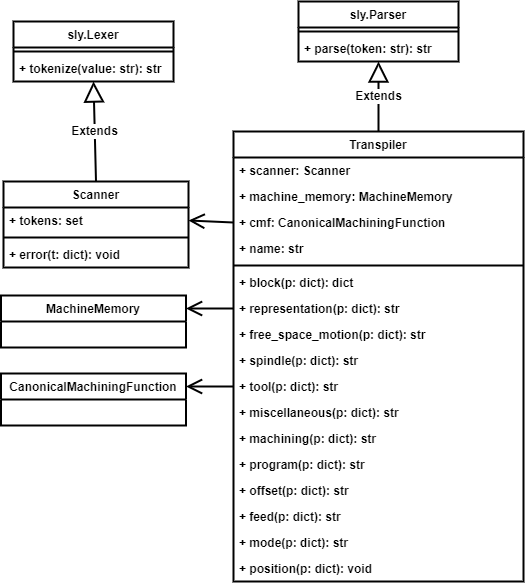
\includegraphics[width=4.5cm]{ncparser-class-transpiler.png}
%     \end{subfigure}
%     %\qquad
%     \begin{subfigure}[b]{0.8\textwidth}
%       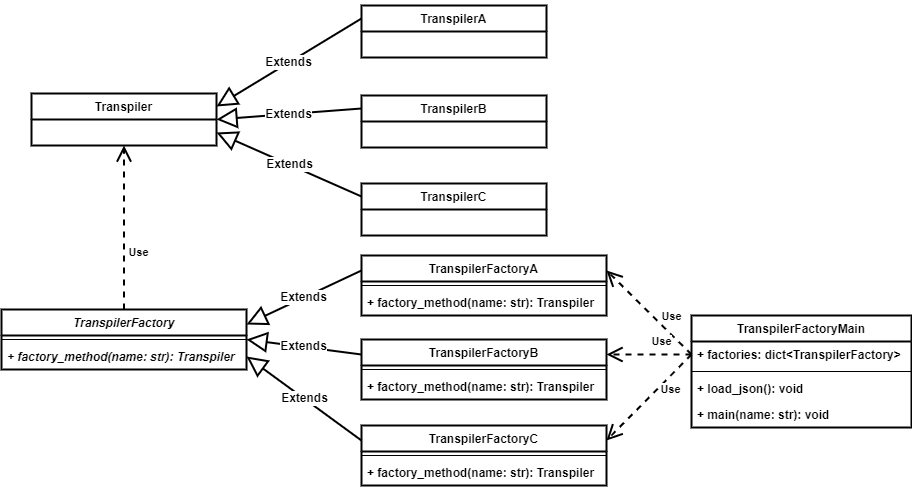
\includegraphics[width=6.5cm]{ncparser-class-transpiler-factory.png}        
%     \end{subfigure}
%     %\caption{Diagrama de Classes}
% \end{figure}


% \subsection{Resultados esperados}
% \begin{frame}{Resultados esperados}
%   \begin{itemize}
%     \item Implementar uma camada abstrata para o registro temporal dos eventos decorrentes do 
%     processamento do programa de controle num\'erico.
%     \item Implementar um aplicativo para o processamento de dialetos de programas de controle 
%     num\'erico industriais.
%     \item Publicar artigo em anais de congressos cient\'ificos.
%     \item Publicar artigo em revista cient\'ifica.
%     \item Fazer o registro do software desenvolvido.
%   \end{itemize}
% \end{frame}




% \subsection{Resultados já alcançados}
% \begin{frame}{Resultados já alcançados}
%   \begin{itemize}
%     \item {
%       A metodologia para a transpila\c c\~ao do arquivo CN para as Fun\c c\~oes Can\^onicas de Usinagem 
%       foi publicada em um artigo cient\'ifico para o 26\textordmasculine Congresso Internacional de 
%       Engenharia Mec\^anica (COBEM 2021), realizado entre os dias 22 e 26 de Novembro de 2021.
%       O t\'itulo do artigo publicado foi \emph{Transpilation from NC Files to Canonical 
%       Machining Functions}.
%     }
%     \item {
%       Outro resultado j\'a alcan\c cado, no contexto do projeto proposto, foi a contribui\c c\~ao no 
%       trabalho do mestrando Vin\'icius Otto Mehl, com o t\'itulo 
%       \emph{Avalia\c c\~ao em tempo real da efetividade global de uma linha de usinagem do tipo transfer}.
%     }
%   \end{itemize}
% \end{frame}


% \subsection{Estudo de Caso}

% \begin{frame}{Objetivos Específicos}
%   \begin{itemize}
%     \item {
%       Interpretar programas de controle num\'erico, escritos em um determinado dialeto do 
%       padr\~ao RS-274D, e convert\^e-los para um outro nível de abstração:
%       \begin{itemize}
%         \item Formato Padronizado;
%         \item Capaz de descrever cada movimento feito durante a usinagem.
%       \end{itemize}
%     }
%     \item {
%       Modelar os \emph{features} de usinagem a partir de um projeto orientado a objetos.
%     }
%     \item {
%       Processar os arquivos de Fun\c c\~oes Can\^onicas de Usinagem e extrair os dados 
%       temporais.
%     }
%   \end{itemize}
% \end{frame}


% Placing a * after \section means it will not show in the
% outline or table of contents.

% \section*{Summary}

% \begin{frame}{Summary}
%   \begin{itemize}
%   \item
%     The \alert{first main message} of your talk in one or two lines.
%   \item
%     The \alert{second main message} of your talk in one or two lines.
%   \item
%     Perhaps a \alert{third message}, but not more than that.
%   \end{itemize}
  
%   \begin{itemize}
%   \item
%     Outlook
%     \begin{itemize}
%     \item
%       Something you haven't solved.
%     \item
%       Something else you haven't solved.
%     \end{itemize}
%   \end{itemize}
% \end{frame}


% All of the following is optional and typically not needed. 
  % \appendix
  % \section<presentation>*{\appendixname}
  % \subsection<presentation>*{For Further Reading}

  % \begin{frame}[allowframebreaks]
  %   \frametitle<presentation>{For Further Reading}
      
  %   \begin{thebibliography}{10}
      
  %   \beamertemplatebookbibitems
  %   % Start with overview books.

  %   \bibitem{Author1990}
  %     A.~Author.
  %     \newblock {\em Handbook of Everything}.
  %     \newblock Some Press, 1990.
  
      
  %   \beamertemplatearticlebibitems
  %   % Followed by interesting articles. Keep the list short. 

  %   \bibitem{Someone2000}
  %     S.~Someone.
  %     \newblock On this and that.
  %     \newblock {\em Journal of This and That}, 2(1):50--100,
  %     2000.
  %   \end{thebibliography}
  % \end{frame}

  % }
